\documentclass[aspectratio=169, 10pt]{beamer}

\usetheme{metropolis}
\usepackage{appendixnumberbeamer}

\usecolortheme[snowy]{owl}

\usepackage{booktabs}
\usepackage[scale=2]{ccicons}

\usepackage{pgfplots}
\usepgfplotslibrary{dateplot}

\usepackage{xspace}
\newcommand{\themename}{\textbf{\textsc{metropolis}}\xspace}
\usepackage{subcaption}

\usepackage[numbers]{natbib}

\title{ImageNet Classification with Deep Convolutional
Neural Networks}
\author{
\vspace{5pt}
\textbf{Guided by,}\\
Abhishek Viswakumar,\\
Assistant Professor\\
Dept. of Electronics and Communication\\
RSET}
\subtitle{Sidharth S\\
S7 ECE Gamma}
\date{\today}

\institute{Rajagiri School of Engineering and Technology}
% \titlegraphic{\hfill\includegraphics[height=1.5cm]{logo.pdf}}

\begin{document}

\maketitle % prints title page
\metroset{block=fill, titleformat=smallcaps}

%%%%%%%%% Slide 1

\begin{frame}
\frametitle{Introduction}
\begin{itemize}
\item AlexNet
\item One of the most influential papers published in computer vision.
	\begin{itemize}
	\item  AlexNet paper has been cited over 70,000 times according to Google Scholar.
	\end{itemize}
\item The network achieved a top-5 error of 15.3\% in ImageNet Large-Scale Visual Recognition Challenge
(ILSVRC) .
\item It is the first Convolutional Neural Network (CNN) where multiple convolution operations were used.
\end{itemize}


\end{frame}

%Slide 2
\begin{frame}
	\frametitle{Abstract}
	\begin{itemize}
		\item Deep convolutional neural network to classify the 1.2 million
high-resolution image.
		\item 60 million parameters and 650,000 neurons.
		\item 1000 class image classification.
		\item Convolutional Layers, Maxpooling layers, Fully connected layers and Softmax layer.
		\item ReLU activation function is used.
		\item GPU implementation of the convolution operation.
		\item Dropout regularization.
	\end{itemize}

\end{frame}

\section{A Short Introduction to Convolutional Neural Networks}

%Slide3
\begin{frame}
	\frametitle{Problem With Fully Connected Networks}
	\begin{block}{Fully Connected Neural Networks}
	\emph{Fully connected neural networks (FCNNs)} are a type of neural network where the architecture is such that all the nodes, or neurones, in one layer are connected to the neurones in the next layer. 
	\end{block}
	For a $64 x 64 x 3$ image,\\
	No of parameters in input layer = $12,288$
	\\
	\vspace{4pt}
	For a $225x225x3$ image,\\
	No of parameters in input layer = $151,875$
	\begin{itemize}
		\item Networks having large number of parameter face several problems, for 				e.g. slower training time, chances of overfitting e.t.c.
	\end{itemize}

\end{frame}

%Slide 4

\begin{frame}
	\frametitle{Convulutional Neural Networks (CNN)}

	\begin{block}{Convolution}
		In mathematics, \alert{convolution} is a mathematical operation on two 					functions $f$ and $g$ that produces a third function $f * g$ that expresses 			how the shape of one is modified by the other.
	\end{block}
 	
	\begin{itemize}
		\item The main image matrix is reduced to a matrix of lower dimension in the first layer itself
		\item  The role of the ConvNet is to reduce the images into a form which is easier to process, without losing features which are critical for getting a good prediction.
	\end{itemize}
		
\end{frame}

%Slide 5
\begin{frame}
	\frametitle{How Convolution is performed}
	We can use an input image and a filter to produce an output image by convolving the filter with the input image.\\
	\vspace{5pt}
	\textbf{Steps:}
	
	\begin{enumerate}
		\item Overlaying the filter on top of the image at some location.
		\item Performing \textbf{element-wise multiplication} between the values in the filter and their corresponding values in the image.
		\item Summing up all the element-wise products. This sum is the output value for the destination pixel in the output image.
		\item Repeating for all locations.
	\end{enumerate}
	
\end{frame}

%Slide 6
\begin{frame}
	\frametitle{Convolution Example}
	\begin{figure}
		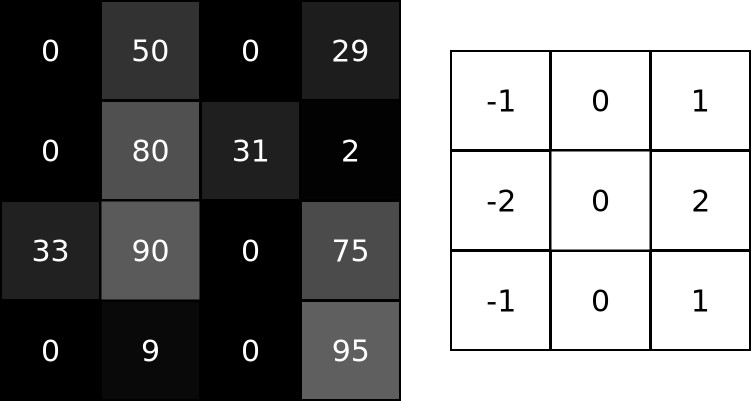
\includegraphics[scale=0.22]{convexample1}
		%\centering \
		\caption{\begin{small}
		A 4x4 image (left) and a 3x3 Sobel filter (right)
		\end{small}}
		%\vspace{3pt}
	\end{figure}
	\vspace{8pt}
Each filter actually happens to be a collection of kernels, with there being one kernel for every single input channel to the layer, and each kernel being unique.
\end{frame}

%Slide7
\begin{frame}

	\frametitle{Convolution Example}
	\begin{figure}[ht]
		\begin{subfigure}{.5\textwidth}
  		\centering
  		% include first image
  		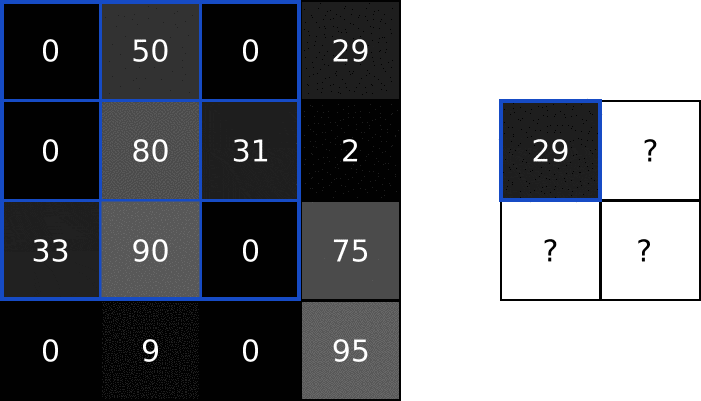
\includegraphics[width=.8\linewidth]{so-0}  
  
		\end{subfigure}

		\begin{subfigure}{.5\textwidth}
  		\centering
  		% include second image
  		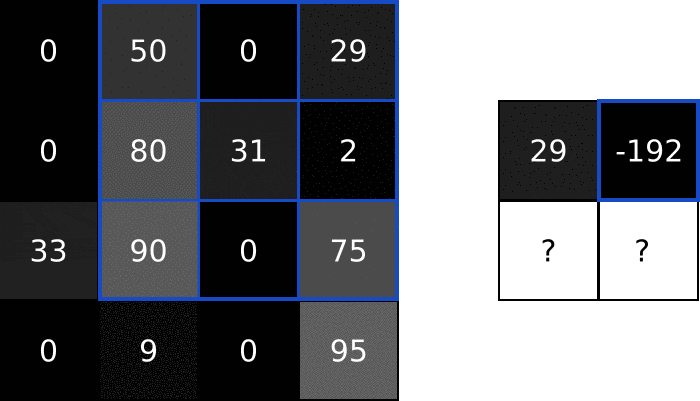
\includegraphics[width=.8\linewidth]{so-1}
		\end{subfigure}
	\caption{Example of Convolution}

\end{figure}
\end{frame}

%slide8
\begin{frame}

	\frametitle{Convolution Example}
	\begin{figure}[ht]
		\begin{subfigure}{.5\textwidth}
  		\centering
  		% include first image
  		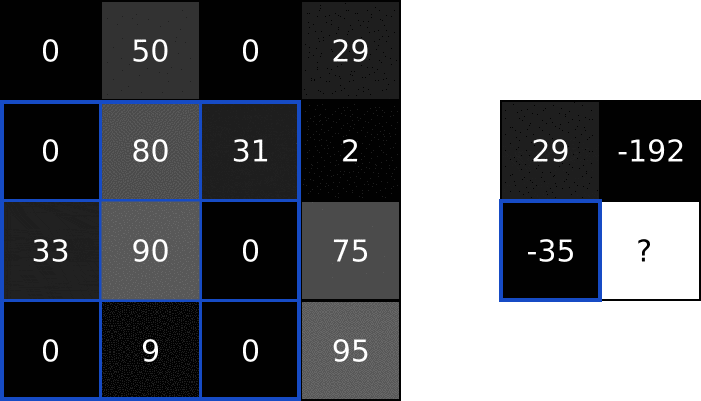
\includegraphics[width=.8\linewidth]{so-2}  
  
		\end{subfigure}

		\begin{subfigure}{.5\textwidth}
  		\centering
  		% include second image
  		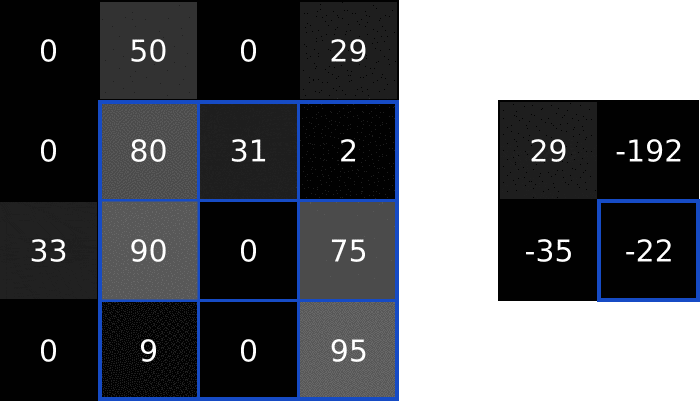
\includegraphics[width=.8\linewidth]{so-3}
		\end{subfigure}
	\caption{Example of Convolution}

\end{figure}
\end{frame}

%%%%%%%%%%%% Slide 9

\begin{frame}
	\frametitle{Kernals/Filters}
	\begin{itemize}
		\item \textit{Sobel filters} are edge-detectors.
		\item Kernals can detect features on a global scale, anywhere in the image.
		\item Kernals to find certain features can be learned using machine learning.
		\item Convolution helps us look for specific localized image features (like edges) that we can use later in the network.
		\item \textbf{Learn new filters} to classify certain features
	\end{itemize}
	
\begin{figure}
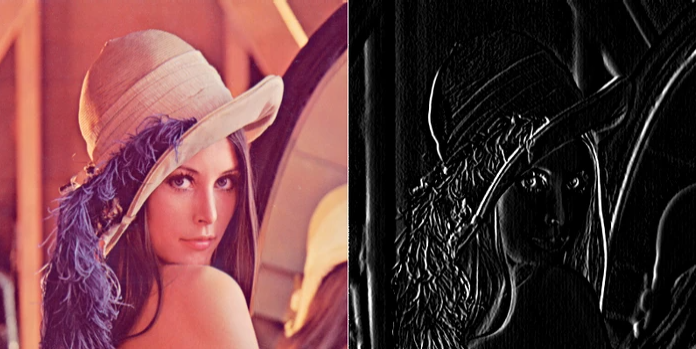
\includegraphics[scale=0.4]{filter}
\centering \
\caption{An image convolved with the vertical Sobel filter}
%\vspace{3pt}
\end{figure}
\end{frame}

%%%%%%%%%%%%%%%%%%% Slide10

\begin{frame}
	\frametitle{MaxPool Layers}
	\begin{itemize}
		\item Neighboring pixels in images tend to have similar values, redundant information.
		\item Reduce the spatial dimension of the input volume for next layers.
	\end{itemize}
	
	\begin{figure}
	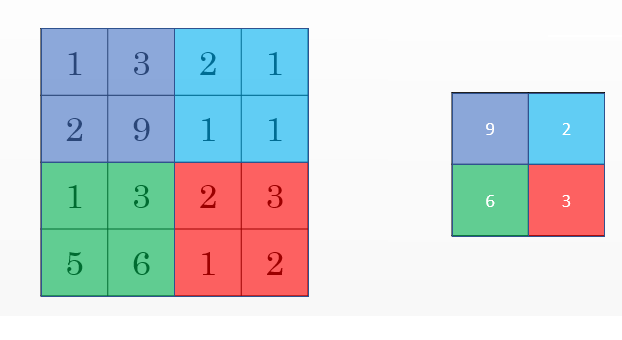
\includegraphics[scale=0.3]{maxpool}
	%\centering \
	\caption{Maxpooling Example}
	%\vspace{3pt}
	\end{figure}
	\begin{itemize}
		\item The max pooling is saying, if the feature is detected anywhere in this filter then keep a high number.
		\item No parameters to learn.
	\end{itemize}
	
\end{frame}

%%%%%%%%%%%%%%%%%%% Slide 11

\begin{frame}
	\frametitle{Padding and Stride}
	
	\begin{block}{Padding}
		\begin{itemize}
			\item If a matrix $nxn$ is convolved with $fxf$ filter/kernel give us $ n-f+1 x n-f+1$ matrix.
			\item Shrinks output.
			\item Throws away a lot of information that are in the edges.
		\end{itemize}
		To solve these problems we can pad the input image before convolution by adding some rows and columns to it. $p$ rows and columns are padded to the input image. 
		\begin{figure}
		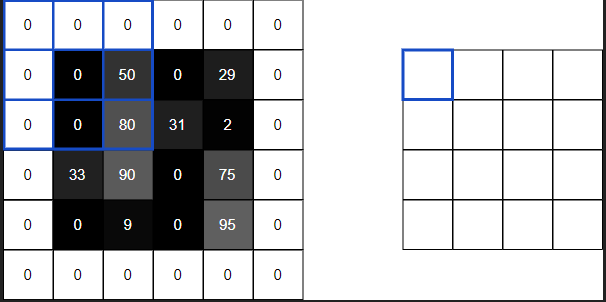
\includegraphics[scale=0.35]{padding}
		%\centering \
		\caption{Padding the input}
		%\vspace{3pt}
		\end{figure}
		
	\end{block}
	
	
	

\end{frame}

%%%%%%%%%%%%%%%%%%%%% Slide 12
\begin{frame}
	\frametitle{Convolution Result}
	
	\begin{block}{Stride}
		Stride $s$ tell us the number of pixels we will jump when we are convolving filter/kernel.
	\end{block}
	For a layer l of a ConvNet,\\
	$f[l]$ = filter size\\
	$p[l]$ = padding\\
	$s[l]$ = stride\\
	$n_{c}[l]$ = number of filters, Then,\\
	\vspace{8pt}
	\begin{block}{Size of output layer}
		When a layer is convolved with filter of size $\displaystyle f[l]\ x\ f[l]\ x\ n_c[l-1]$\\
		Output size is $n[l]\ x\ n[l]\ x\ n_c[l]$ where,\\
		\vspace{6pt}
		$n[l] = \displaystyle \frac{n[l-1] + 2p[l] - f[l]}{s[l]} + 1$\\
		\vspace{6pt}
		$n_c[l]$ = Number of filters used.
		
		
	\end{block}

\end{frame}

\section{AlexNet}

%%%%%%%%%%%%  Slide 13
\begin{frame}
	\frametitle{Architecture of AlexNet}
	
	\begin{figure}
	\centering
	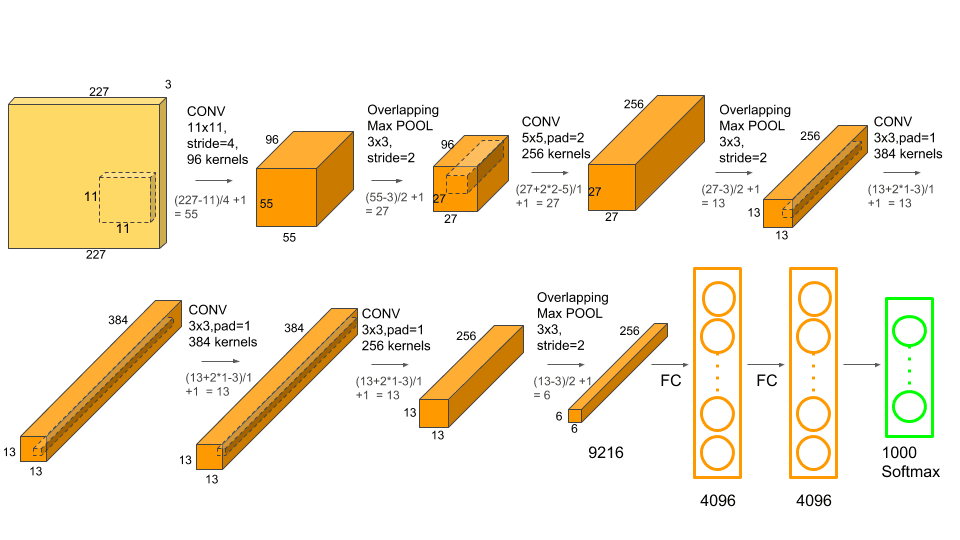
\includegraphics[scale=0.36]{architecture}
	%\centering \
	\caption{Architecture of AlexNet}
	%\vspace{3pt}
	\end{figure}

\end{frame}

%%%%%%%%%%%%%%% Slide 14
\begin{frame}
	\frametitle{Arhitecture of AlexNet}
	
	\begin{itemize}
		\item 8 learned layers
		\begin{itemize}
			\item Five convolutional and three fully-connected.
		\end{itemize}
		\item Final layer is softmax layer which can classify 1000 classes
		\item $\sim 60$ million parameters.
		\item Trained on ImageNet dataset.
		\item Uses ReLU nonlinearity for activation.
	\end{itemize}

\end{frame}

%%%%%%%%%%%%%%%% Slide 15
\begin{frame}
	\frametitle{ReLU Nonlinearity}
	\vspace{5pt}
	\emph{What is an activation function?}
	\vspace{8pt}
	
	\begin{itemize}
		\item Decides whether a neuron should fire or not.
		\item Helps the network learn complex patterns in data.
		\item Takes output of previous layer and converts it to meaningful form to transfer to next layer as input.
	\end{itemize}
	
	\vspace{8pt}
	
	\emph{Why do we need activation functions?}
	\vspace{8pt}
	
	\begin{itemize}
		\item Output value of a layer is restricted to a limit.
		\item Ability to add \textbf{nonlinearity} into a neural network.
		\item Allows back propagation and gradient descent to update the weights in the network.
	\end{itemize}
	
	\vspace{5pt}
	Some examples of activation functions are: \textit{Sigmoid, tanh, ReLU, Linear}
\end{frame}

%%%%%%%%%%%%%%%% Slide 16
\begin{frame}
	\frametitle{ReLU Nonlinearity}
	\begin{columns}
		\begin{column}{0.5\textwidth}
			\begin{block}{ReLU Activation} 
				\[ f(x) =
  				\begin{cases}
    			0       & \quad \text{for } x\ <\ 0\\
    			x  & \quad \text{for } x\ \geq\ 0
  				\end{cases}
				\]
			\end{block}
			
			\begin{itemize}
				\item Deep convolutional neural networks with ReLUs train several times faster than their
equivalents with tanh units.
				\item Easier to train.
				\item Better for learning complex relationships.
			\end{itemize}
			
		\end{column}
		
		\begin{column}{0.5\textwidth}
			\begin{figure}
				\begin{center}
					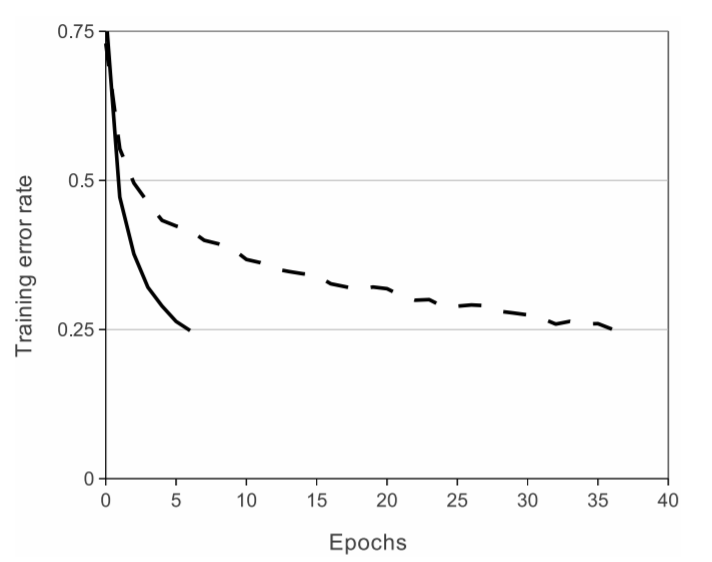
\includegraphics[scale=0.4
					]{relu}
					\caption{A four-layer convolutional neural
network with ReLUs \textbf{(solid line)} reaches a 25\%
training error rate on CIFAR-10 six times faster
than an equivalent network with tanh neurons
\textbf{(dashed line)}.}
				\end{center}
			\end{figure}
		\end{column}
		
	\end{columns}
				
\end{frame}

%%%%%%%%%%%%%%%%%% Slide 17
\begin{frame}
	\frametitle{Dataset and GPUs}
	%\begin{block}{ImageNet}
	\textbf{ImageNet Dataset}
		\begin{itemize}
			\item 15 million high-resolution images labeled with 22 thousand classes.
			\item ImageNet Large-Scale Visual Recognition Challenge (ILSVRC).
			\item 1.2 million training images, 50 thousand validation images, and 150 thousand testing images.
			\item Authors used downsampled 227 x 227 images.
		\end{itemize}
	
	%\end{block}
	\vspace{8pt}
	\textbf{Training on GPUs}
%	\begin{block}{Use of multiple GPUs}
		\begin{itemize}
			\item GPUs are faster and efficient for matrix multiplication and convolution.
			\item CPUs are latency optimized. GPUs are bandwidth optimized.
			\item AlexNet allows for multi-GPU training by putting half of the model’s neurons on one GPU and the other half on another GPU.
		\end{itemize}
%	\end{block}

\end{frame}

%%%%%%%%%%%%%% Slide 18
\begin{frame}
	\frametitle{Softmax Layer}
	
	\begin{block}{Softmax Function}
		\[ softmax(\overrightarrow{Z})_i = \frac{exp(z_i)}{\sum_{j}^{K}exp(z_j))}\]
		\vspace{10pt}\\
		$\overrightarrow{Z}$ The input vector to the softmax function, made up of (z0, ... zK)\\
		$z_i$  elements of the input vector to the softmax function
	\end{block}
	
	\begin{itemize}
		\item Used for multiclass classification/regression.
		\item The Softmax regression is a form of logistic regression that normalizes an input value into a vector of values that follows a probability distribution whose total sums up to 1.
		
	\end{itemize}

\end{frame}

%%%%%%%%%%%%% Slide 19
\begin{frame}
	\frametitle{Reduce Overfitting}
		\begin{itemize}
			\item Overfitting refers to a model that models training data too well.
			\item Happens when a model learns the detail and noise in the training data to the extent that it negatively impacts the performance of the model on new data.
		\end{itemize}
	
	\begin{figure}
				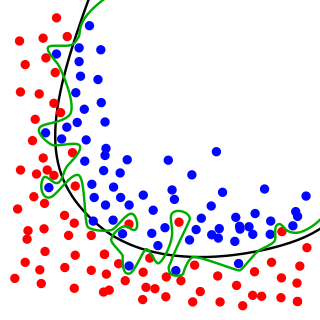
\includegraphics[scale=0.3]{overfit}
				%\centering \
				\caption{Black line fits the data well. Green is overfitting.}
				%\vspace{3pt}
			\end{figure}		
			
		Overfitting can be reduced by: Getting more training data, Regularization.

\end{frame}

%%%%%%%%%%%%% Slide 20
\begin{frame}
	\frametitle{Dropout Regularization}
	
	\begin{itemize}
		\item Sets to zero the output of each hidden neuron with probability 0.5.
		\item  The neurons which are “dropped out” do not contribute to the forward pass and do not participate in backpropagation.
		\item This technique reduces complex co-adaptations of neurons.
		\item  Network is forced to learn more robust features.
		\item Employs dropout in the first two fully-connected layers of the network.
		\item \textit{"Without dropout, our network exhibits substantial overfitting."}
		\item Dropout increases number of iterations required to train the network.
	\end{itemize}
\end{frame}

%%%%%%%%%%%%%%% Slide 21
\begin{frame}
	\frametitle{Details of Learning}
	\begin{itemize}
		\item Trained using stochastic gradient descent with batch size = 128.
		\item Momentum 0.9 and weight decay of 0.0005.
		\item Small amount
of weight decay was important for the model to learn.
		
	\end{itemize}
	\begin{figure}
		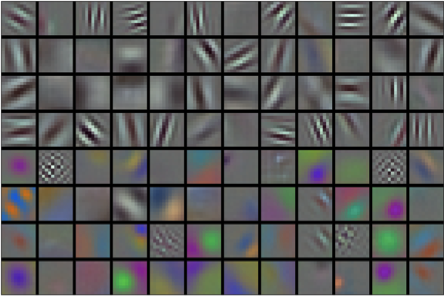
\includegraphics[scale=0.3]{learning}
		\centering
		\caption{96 convolutional kernels of size
11×11×3 learned by the first convolutional
layer on the 224×224×3 input images.}
		%\vspace{3pt}
	\end{figure}

\end{frame}

%%%%%%%%%%%%%% Slide 22
\begin{frame}
	\frametitle{Results}
	\begin{itemize}
		\item The network achieves top-1 and top-5 test set error rates of 37.5\% and 17.0\% in ILSVRC - 2010.
		\begin{itemize}
			\item Next best result is  45.7\% and 25.7\% respectively.
		\end{itemize}
		\vspace{8pt}
		
		\begin{center}
		\begin{table}
		\begin{tabular}{||c| c| c||} 
	 	\hline
 		\textbf{Model} & \textbf{Top-1} & \textbf{Top-5} \\ [0.5ex] 
 		\hline\hline
 		\textit{Sparse Coding} & \textit{47.1\%} & \textit{28.2\%}\\ 
 		\hline
 		\textit{SIFT + FVs [24]} & \textit{45.7\%} & \textit{25.7\%} \\
 		\hline
 		CNN & \textbf{37.5\%} & \textbf{17.0\%}\\
 		\hline
 	\end{tabular}
 	\caption{Comparison of results on ILSVRC-2010 test set. In italics are best results
achieved by others.}
	\end{table}
	\end{center}

		\item The CNN described in this paper achieves
a top-5 error rate of 18.2\% in ILSVRC - 2012.
		\begin{itemize}
			\item The second-best contest entry achieved an error rate of 26.2\%.
		\end{itemize}
	\end{itemize}

\end{frame}

%%%%%%%%%%%%%Slide 23
\begin{frame}
	\frametitle{Result}
	\begin{figure}
		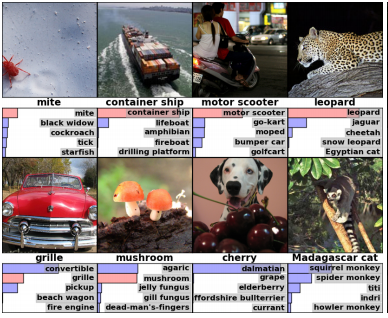
\includegraphics[scale=0.6]{result}
		%\centering \
		\caption{Eight ILSVRC-2010 test images and the five labels considered most probable by the model. The correct label is written under each image, and the probability assigned to the correct label is also shown with a red bar (if it happens to be in the top 5).}
		%\vspace{3pt}
	\end{figure}

\end{frame}

%%%%%%%%%%Slide 24
\begin{frame}
	\frametitle{Conclusion}
	\begin{itemize}
		\item AlexNet was the pioneer in CNN and open the whole new research era.
		\item Dropout, ReLU, and deep layers are key steps in achieving excellent performance in computer vision tasks.
		\item Removing any of the convolutional layers will drastically degrade AlexNet’s performance.
		
	\end{itemize}
	\vspace{8pt}
	\textbf{Comparison:}
	\begin{itemize}
	\item \textit{GoogleNet}: Winner of the ILSVRC 2014 competition was GoogleNet from Google. Achieved top-5 error rate of 6.67\%.\\
	\item \textit{ResNet}: Winner, ILSVRC 2015. Introduced a novel architecture with "skip connections". Achieves a top-5 error rate of 3.57\% which beats human-level performance on this dataset.
	
	\end{itemize}
	
\end{frame}

\begin{frame}
	\vspace{20pt}
	\nocite{7820046}
	\nocite{krizhevsky2017imagenet}
	\nocite{he2016deep}
	
	\bibliographystyle{IEEEtraN}
	\bibliography{cite}
	
\end{frame}

\begin{frame}[t]{}\vspace{5pt}
\vspace{90pt}
\centering

\Huge THANK YOU
\end{frame}







\end{document}
%%%%%%%%%%%%%%%% Slide 25
%\begin{frame}[t]{References}\vspace{20pt} 
%
%[1].M. W. Guo, J. S. Wang, L. F. Zhu, S. S. Guo and W. Xie, "An Improved Grey Wolf Optimizer Based on Tracking and Seeking          Modes to Solve Function Optimization Problems," in IEEE Access, vol. 8, pp. 69861-69893, 2020\vspace{5pt}\newline
%[2].Mirjalili, S., Mirjalili, S. M., Lewis, A. (2014). Grey wolf optimizer. Advances in engineering software, 69, 46-61\vspace{5pt}\newline
%\end{frame}

\end{document}